\documentclass{pj}

\usepackage{hyperref}
\usepackage{cite}
\usepackage{amsmath}
%\interdisplaylinepenalty=2500 % suggested by IEEE to use with amsmath package
\usepackage{amsfonts}
\usepackage{graphicx}
\usepackage{subfigure}
\usepackage{epstopdf}

\usepackage[T1]{fontenc} % optional
\usepackage[cmintegrals]{newtxmath}
\usepackage{bm} % optional

% correct bad hyphenation here
\hyphenation{op-tical net-works semi-conduc-tor}

\begin{document}
\setcounter{page}{1}
\pjheader{}

\title{Analysis of Waveguide using Finite Element Method}
%\maketitle

\newcommand{\defaultfigurewidth}{0.5\columnwidth}

\footnote{\hskip-0.12in*\ Chang-Pao Chang (cchang95@uiuc.edu).}
\footnote{\hskip-0.12in\textsuperscript{1} University of Illinois at Urbana-Champaign, Urbana, Illinois, 61801}

\author{Chang-Pao Chang\textsuperscript{*,1}}



\begin{abstract}
	This paper demonstrated a full-wave analysis of waveguide structure using finite element method (FEM). Vector formulation and edge basis are used to avoid the spurious mode. Several common homogeneous waveguide structure such as rectangular, cylindrical are used to demonstrate the correctness of the FEM code. Finally, the metal-insulator-semiconductor structure, a common waveguide used extensively in silicon process, are analyzed.
\end{abstract}
%
\section{introduction}
\label{sec:Intro}
The guidance condition of waveguide have been a interesting problem in various field, such as millimeter wave or optical component design. However, only some specific waveguide structure have analytic solution. Therefore, the numerical analysis of waveguide becomes important. \\


Different numerical methods have been proposed and used to solve this problems. However, the finite element method shines beyond others. The finite element method (FEM) has advantage over other numerical methods because of its highly localized element property. Therefore, FEM becomes a popular method in solving this problem. However, the nodal basis will have spurious mode \cite{na_JinJM_JinJM_2014_finite_element}, and require artificially remove those modes. Fortunately, the development of edge element combined with vector functional provide a good way to overcome this problems.\\


After the discretization of the waveguide cross section into a number of triangles, the vector functional and Galerkin method is applied. Edge basis is used to expand the transverse electric field, while nodal basis is used to represent the longitudinal electric field.\\

One waveguide used widely in semiconductor industry is metal-insulator-semiconductor (MIS) structure \cite{ITMTT_KiangJF_KiangJF_1996_quasitem_analysis,ITMTT_WilliamsDF_WilliamsDF_1999_metalinsulatorsemiconductor_transmission}. During the low frequency around kilo-hertz, the semiconductor is regarded as a good conductor. However, over several mega hertz, when the minority carrier in space charge region can not follow the fast sweeping voltage, the semiconductor can be simplified as a lossy material. However, the presence of insulator makes the entire guidance condition very different from traditional microstrip. \\


This paper is organized as follow. In Sec.~\ref{sec:Formulation} will be briefly introduced. Several homogeneous waveguide are used to demonstrate the correctness of the code in Sec.~\ref{sec:homo_wg}. Two more examples are given in \ref{sec:inhomo_wg} to show the capability of inhomogeneous waveguide. Finally, three different modes of fundamental guided wave of MIS structure will be given as an numerical example.\\

\section{Formulation}
\label{sec:Formulation}
\subsection{Vector Helmholtz Equation}
Start from Maxwell's equation in frequency domain by assume the harmonic variation ${e}^{j \omega t}$, we have
\begin{eqnarray}
\nabla \times \mathbf{E} &=& -j \omega \mu \mathbf{H} \label{maxwell_1}\\
\nabla \times \mathbf{H} &=& \sigma \mathbf{E} + j \omega \epsilon \mathbf{E} = j \omega \bar{\epsilon} \mathbf{E}, 
\label{maxwell_2}
\end{eqnarray}
where $\bar{\epsilon} = \epsilon + {\sigma}/{j \omega}$ is the equivalent complex permittivity, and $\sigma$ is the electrical conductivity. The vector Helmholtz equation can therefore be obtain from (\ref{maxwell_1}) and (\ref{maxwell_2}), 
\begin{equation}
\nabla \times \left( \frac{1}{\mu_r} \nabla \times \mathbf{E} \right) - {k_0}^2 \bar{\epsilon_r} \mathbf{E} = 0
\label{eq:helm}, 
\end{equation}
where $k_0 = \omega \sqrt{\mu_0 \epsilon_0}$ is the propagation constant in vacuum, and $\bar{\epsilon_r} = \bar{\epsilon} / \epsilon_0$ is the relative permittivity. 

By assuming the that all field propagating along z direction, with dependency of $e^{-\gamma z}$, and decomposing the transverse and longitudinal field, the electric field in (\ref{eq:helm}) can be written as,
%
\begin{equation}
\mathbf{E}(x, y, z) = \left \{ \mathbf{E_t}(x,y) + E_z(x,y) \right \} e^{-\gamma z} \nonumber
\end{equation}
%
The del-operator $\nabla$ can also be decomposed to transverse del-operator $\nabla_t$ and partial derivative along z $\partial / \partial z$,
\begin{eqnarray}
\nabla = \nabla_t - \hat{z} \frac{\partial}{\partial z}  = \nabla_t -\gamma \hat{z}.
\nonumber
\end{eqnarray}
%
In \cite{na_JinJM_JinJM_2014_finite_element}, a variable transformation is introduced , 
\begin{eqnarray}
\mathbf{e}_t &=& -j\gamma \mathbf{E}_t \nonumber \\
e_z &=& -jE_z
\label{tranf2}
\end{eqnarray}
%
The resulting boundary condition on PEC is, 
\begin{eqnarray}
\hat{n} \times \mathbf{e}_t &=& 0 \nonumber \\
e_z &=& 0,
\end{eqnarray}
and on PMC,
\begin{eqnarray}
(\nabla_t e_z + \mathbf{e}_t) \cdot \hat{n} &=& 0 \nonumber \\
\nabla_t \times \mathbf{e}_t  &=& 0.
\end{eqnarray}

\subsection{Finite Element formulation}
The functional of this PDE becomes \cite{na_JinJM_JinJM_2014_finite_element},
\begin{eqnarray}
F\left(\mathbf{e}_t,e_z\right) &=& \int_\Omega \bigg[ \frac{1}{\mu_r} (\nabla \times \mathbf{e}_t)
\cdot ( \nabla \times \mathbf{e}_t )^* - k_0^2 \bar{\epsilon_r} \mathbf{e}_t \cdot \mathbf{e}_t^* \bigg]d\Omega \nonumber \\
&-& \gamma^2 \int_\Omega \bigg[ \frac{1}{\mu_r}(\nabla_t e_z + \mathbf{e}_t)\cdot(\nabla_t e_z + \mathbf{e}_t) - k_0^2 \bar{\epsilon_r} e_z e_z^* \bigg] d\Omega.
\label{eq:variation}
\end{eqnarray}

Using the edge basis $\mathbf{N}_i^e$, the transverse field can be represented by,
\begin{equation}
\mathbf{e}_t^e = \sum_{i=1}^{n} \mathbf{N}_i^e e_{ti}^e
\label{et}.
\end{equation}
However, the longitudinal field is expanded by nodal basis $N_i^e$,
\begin{equation}
e_z^e = \sum_{i=1}^n N_i^e e_{zi}^e
\label{ez}
\end{equation}

Substituting this into Fig.~\ref{eq:variation}, one can obtains the generalized eigenvalue problem \cite{na_JinJM_JinJM_2014_finite_element},
\begin{eqnarray}
\bigg[ \begin{matrix} A_{tt}&0\\ 0&0 \end{matrix} \bigg] \bigg\{ \begin{matrix} e_t\\ e_z \end{matrix} \bigg\} &=& \gamma^2 \bigg[ \begin{matrix} B_{tt}&B_{tz}\\ B_{zt}&B_{zz} \end{matrix} \bigg] \bigg\{ \begin{matrix} e_t\\ e_z \end{matrix} \bigg\},
\end{eqnarray}
where the matrices are
\begin{eqnarray}
[A_{tt}^e] &=& \int_\Omega \bigg[ \frac{1}{\mu_r^e} \{ \nabla_t \times \mathbf{N}^e \}
\cdot \{ \nabla_t \times \mathbf{N}^e \}^T - k_0^2 \bar{\epsilon_r}^e \{\mathbf{N}^e\} \cdot \{\mathbf{N}^e\}^T \bigg]d\Omega \\
\left[ B_{tt}^e \right] &=& \int_\Omega \frac{1}{\mu_r^e} \{\mathbf{N}^e\} \cdot \{\mathbf{N}^e\}^T d\Omega \\
\left[ B_{tz}^e \right] &=& \int_\Omega \frac{1}{\mu_r^e} \{\mathbf{N}^e\} \cdot \{\nabla_t{N}^e\}^T d\Omega \\
\left[ B_{zt}^e \right] &=& \int_\Omega \frac{1}{\mu_r^e} \{\nabla_t {N}^e\} \cdot \{\mathbf{N}^e\}^T d\Omega \\
\left[ B_{zz}^e \right] &=& \int_\Omega \bigg[ \frac{1}{\mu_r^e} \{ \nabla_t N^e \}
\cdot \{ \nabla_t N^e \}^T - k_0^2 \bar{\epsilon_r}^e \{ N^e \}\{ N^e\}^T \bigg]d\Omega
\label{elemat}
\end{eqnarray}

\section{Homogeneous Waveguide}
\label{sec:homo_wg}
To examine the correctness of the FEM code, two examples of homogeneous cylindrical waveguide is provided, rectangular waveguide and cylindrical waveguide. The analytic solution of these two example were compared with numerical solution. 

\subsection{Rectangular Waveguide}
Fig.~\ref{fig:rect_geom} shows the geometry of the homogeneous rectangular waveguide. The cutoff wavenumber of $\mathrm{TE}_{mn}$ and $\mathrm{TM}_{mn}$ mode can be analytically calculated by,
\begin{eqnarray}
k_{c,mn} = \sqrt{\left( \frac{m \pi}{a}\right) ^2 + \left(\frac{n \pi}{b}\right)^2 }. 
\end{eqnarray}
After obtaining the cutoff frequency, the propagation constant $\beta_z$ can be further obtained,
\begin{equation}
\beta _{z,mn} = \mathrm{Im} \left \{ j\sqrt{k_0^2 - k_{c,mn}^2} \right \}.
\label{eq:rect_beta_z}
\end{equation}

\begin{figure}[htbp]
	\centering
	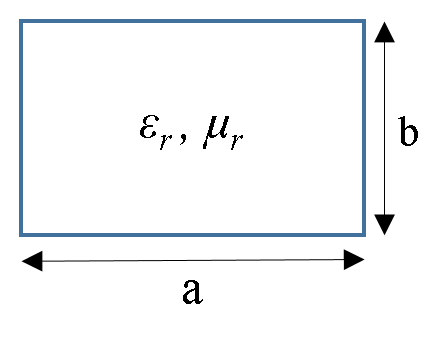
\includegraphics[width=0.3\columnwidth]{./img/rectangular/geometry.png}
	\caption{Geometry of homogeneous rectangular waveguide. }
	\label{fig:rect_geom} % label must put at the last
\end{figure}
\begin{figure}[htbp]
	\centering
	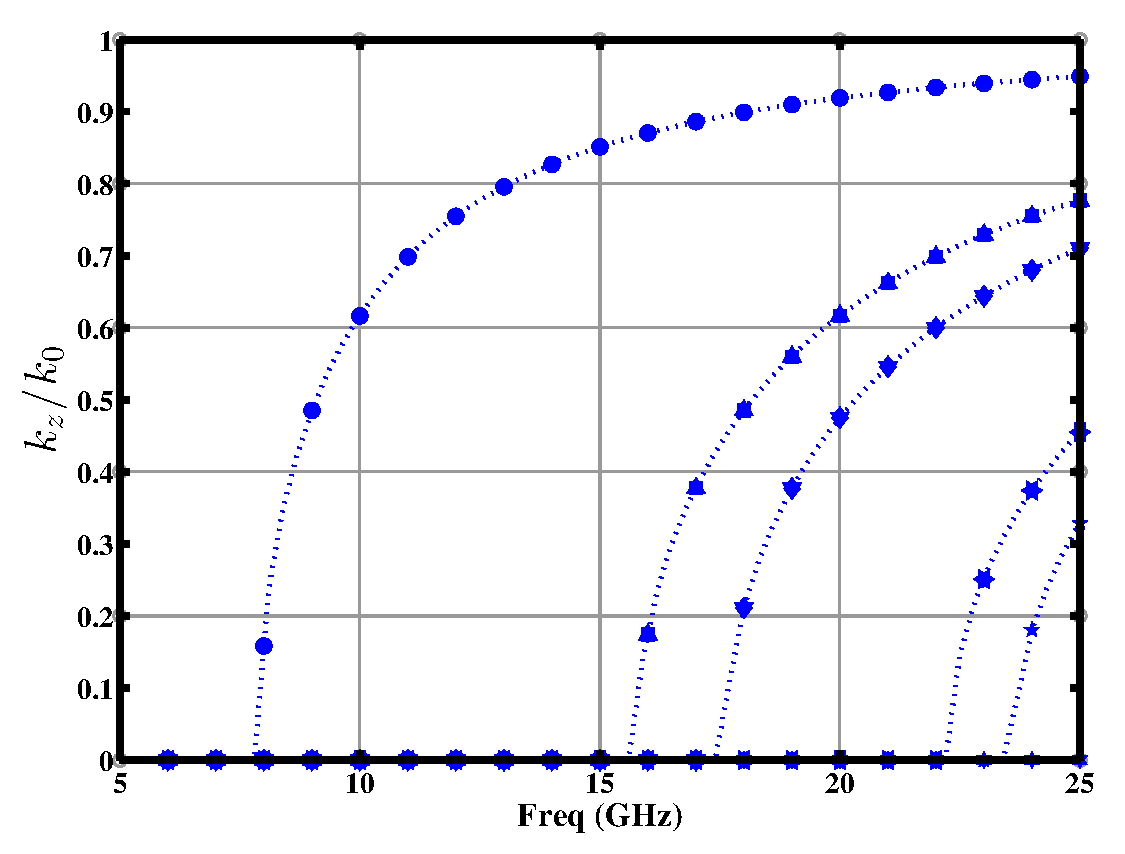
\includegraphics[width=\defaultfigurewidth]{./img/rectangular/dispersion.eps}
	\caption{Dispersion curves for a homogeneous rectangular waveguide. Dash line: exact solution; symbols: numerical solution ($b=a/2=9.525\rm{mm}$, $\mu_r=\epsilon_r=1$).}
	\label{fig:rect_dispersion}
\end{figure}

Fig.~\ref{fig:rect_dispersion} shows the comparison of dispersion curve of WR75 waveguide. The finite element solution is in good agreement with exact solution obtained from (\ref{eq:rect_beta_z}).

\subsection{Cylindrical Waveguide}
Another example of homogeneous cylindrical waveguide is cylindrical waveguide, as shown in Fig.~\ref{fig:cylin_geom}.  The cutoff frequencies of $\mathrm{TE}_{mn}$ mode can be analytically calculated by,
\begin{eqnarray}
k_{c,mn} = \frac{\beta_{mn}}{r},  
\end{eqnarray}
while the cutoff frequencies of $\mathrm{TM}_{mn}$ are
\begin{eqnarray}
k_{c,mn} = \frac{\alpha_{mn}}{r},
\end{eqnarray}
where $\alpha_{mn}$ are the m-th root of n-th order Bessel function of first kind, $J_m(\alpha_{mn})=0$, and $\beta_{mn}$ are the m-th root of the derivative of n-th order Bessel function of first kind, $J_m^\prime(\beta_{mn})=0$. 

\begin{figure}[htbp]
	\centering
	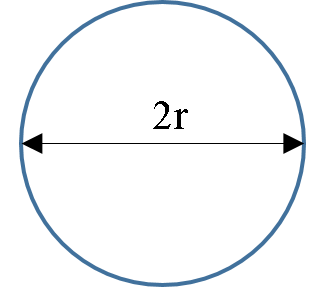
\includegraphics[width=0.3\columnwidth]{./img/cylindrical/geometry.png}
	\caption{Geometry of homogeneous cylindrical waveguide. }
	\label{fig:cylin_geom}
\end{figure}
\begin{figure}[htbp]
	\centering
	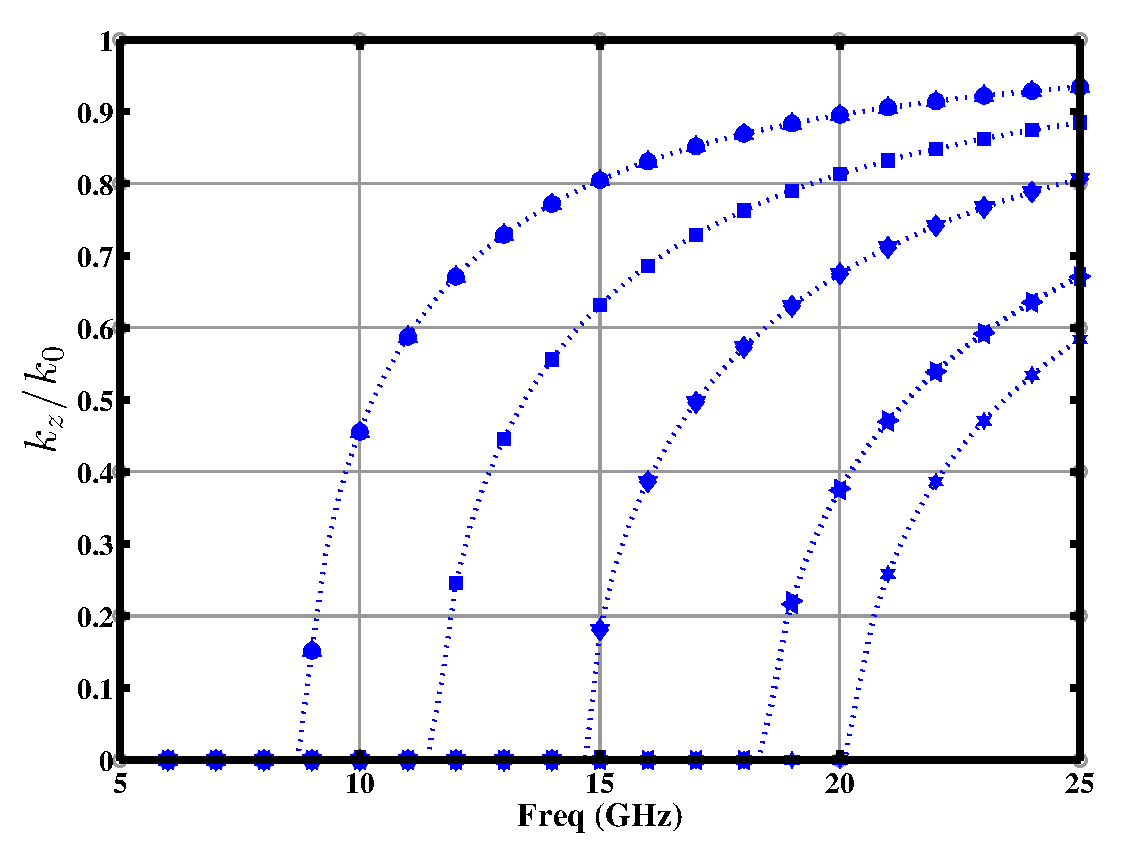
\includegraphics[width=\defaultfigurewidth]{./img/cylindrical/dispersion.eps}
	\caption{Dispersion curves for a homogeneous cylindrical waveguide. Dash line: exact solution; symbols: numerical solution ($r=10\rm{mm}$, $\mu_r=\epsilon_r=1$).}
	\label{fig:cylin_dispersion}
\end{figure}

Fig.~\ref{fig:cylin_dispersion} shows the comparison of dispersion curve of cylindrical waveguide with 10 mm radius. The finite element solution is in good agreement with exact solution obtained from (\ref{eq:rect_beta_z}).

\section{Inhomogeneous Waveguide}
\label{sec:inhomo_wg}
In this section, another two examples are also demonstrated the capability of the same code to obtain the dispersion curve. The first example is partially filled rectangular waveguide, and the second example is the shielded microstrip line enclosed by an partially filled rectangular waveguide. The result of first example is compared with exact solution, and the result of second example is compared with the result obtained from node element in \cite{na_JinJM_JinJM_2014_finite_element}. 

\subsection{Partially filled Rectangular Waveguide}
\label{subsec:rect_inhomo}
The partially filled rectangular waveguide is the rectangular waveguide filled with two different material, as shown in Fig.~\ref{fig:rect_inhomo_geom}. If the material 1 and 2 only differs in permittivity, i.e. $\mu_{r1} = \mu_{r2}$, then the analytic solution can be obtained through separating $\mathrm{TE_{y}}$ and $\mathrm{TM_y}$ \cite{na_CollinRE_CollinRE_1991_field_theory}. In the rest of section, the homogeneity of permeability is assumed, i.e. $\mu_{r1} = \mu_{r2}$.
%
\begin{figure}[htbp]
	\centering
	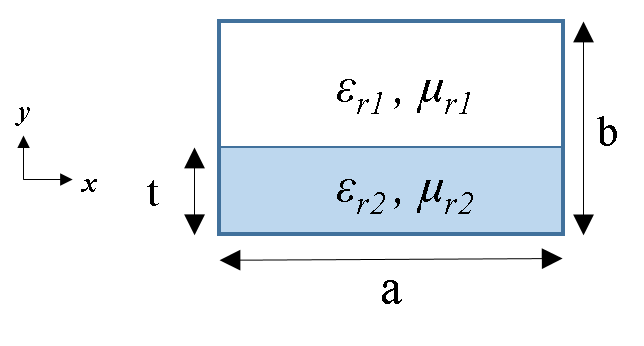
\includegraphics[width=0.5\columnwidth]{./img/rectangular_inhomo/geometry.png}
	\caption{Geometry of partially filled rectangular waveguide. }
	\label{fig:rect_inhomo_geom}
\end{figure}

%In \cite{na_JinJM_JinJM_2014_finite_element}, the numerical solution is carried out through placing the perfect magnetic conductor (PMC) at the symmetry plane with normal vector parallel to x axis.
The $\mathrm{TE_{y}}$, or LSE modes in \cite{na_CollinRE_CollinRE_1991_field_theory}, have analytic solution. The cutoff wavenumber can be obtained by transverse resonance condition \cite{na_CollinRE_CollinRE_1991_field_theory}. Introducing two additional variables $p,q$, 

\begin{eqnarray}
\frac{\mathrm{tan} pt}{p} &=& - \frac{\mathrm{tan} q(b-t)}{q} \nonumber \\
p^2-q^2 &=& k_{1c}^2 \left( \frac{\epsilon_{r2}}{\epsilon_{r1}} - 1\right)
\end{eqnarray}
The cutoff wavenumber can then be obtained through the solution to the previous equation by
\begin{eqnarray}
\gamma = p^2 + \left(\frac{m\pi}{a}\right)^2 - k_1^2\cdot\frac{\epsilon_{r2}}{\epsilon_{r1}} = q^2 + \left(\frac{m\pi}{a}\right)^2 - k_1^2
\label{eq:rect_inhomo_gamma_pq}.
\end{eqnarray}
%
%
%through placing the perfect electric conductor (PEC) at the symmetry. 
Similarly, the $\mathrm{TM_{y}}$, LSM mode, can be analyzed by introducing two additional variables $p,q$, 
\begin{eqnarray}
p\cdot\mathrm{tan} pt &=& - \frac{\epsilon_{r2}}{\epsilon_{r1}}\cdot q\cdot\mathrm{tan} q(b-t) \nonumber \\
p^2-q^2 &=& k_{1c}^2 \left(\frac{\epsilon_{r2}}{\epsilon_{r1}} - 1\right),
\end{eqnarray}
and the cutoff propagation constant can be obtained through same (\ref{eq:rect_inhomo_gamma_pq}).

\begin{figure}[htbp]
	\centering
	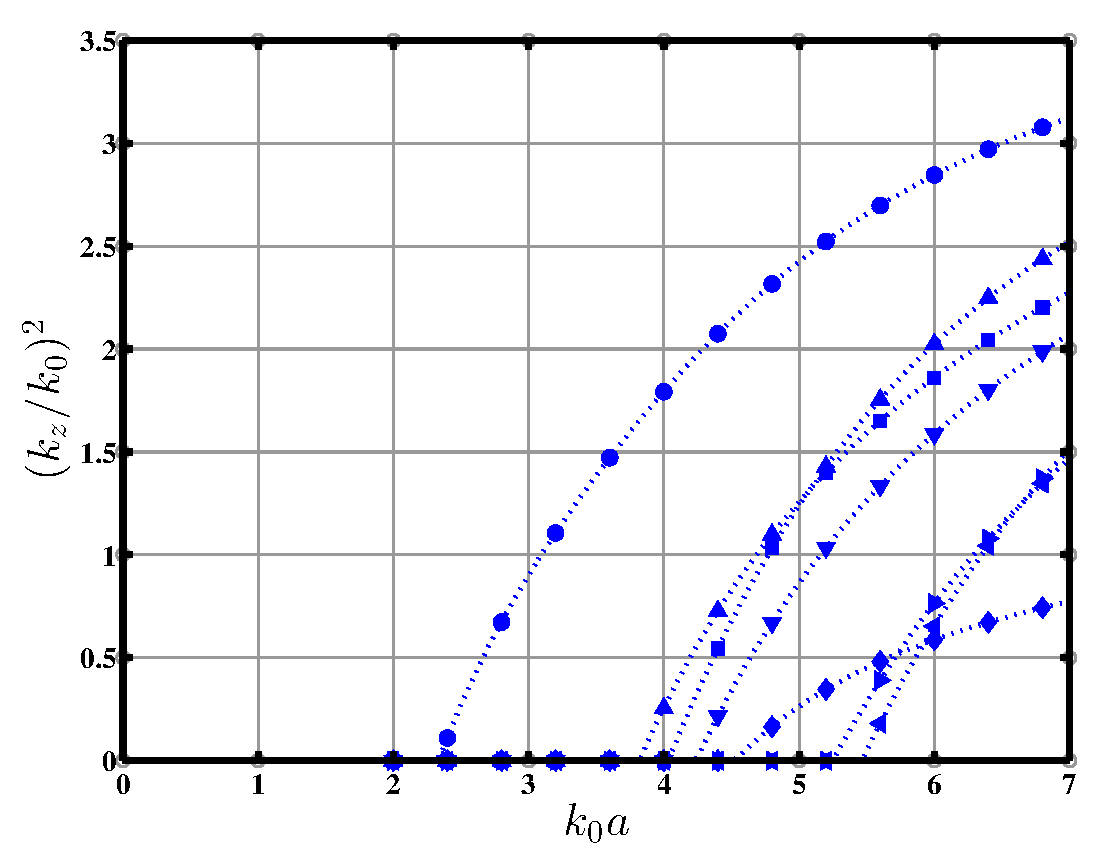
\includegraphics[width=\defaultfigurewidth]{./img/rectangular_inhomo/dispersion.eps}
	\caption{Dispersion curves for a homogeneous cylindrical waveguide. Solid line: exact LSE solution; dash line: exact LSM solution; symbols: numerical solution ($b=a/2$, $t=b/2$, $\mu_{r1}=\mu_{r2}=\epsilon_{r1} = 1$, $\epsilon_{r2} = 4$).}
	\label{fig:rect_inhomo_dispersion}
\end{figure}


\subsection{Shielded Microstrip line Enclosed by Rectangular Waveguide}

The second example for inhomogeneous waveguide is the same waveguide presented in Sec.~\ref{subsec:rect_inhomo} with a piece of strip on the boundary between two material. Fig.~\ref{fig:rect_inhomo_strip_geom} shows the geometry of this shielded waveguide. Fig.~\ref{fig:rect_inhomo_strip_dispersion} shows the comparison between the numerical result and the results obtained from nodal element in \cite{na_JinJM_JinJM_2014_finite_element}. 

%However, one should note that in \cite{na_JinJM_JinJM_2014_finite_element}, a perfect magnetic wall is placed at the symmetry plane of the structure. However, other modes can still exist when the PMC is not present. 

\begin{figure}[htbp]
	\centering
	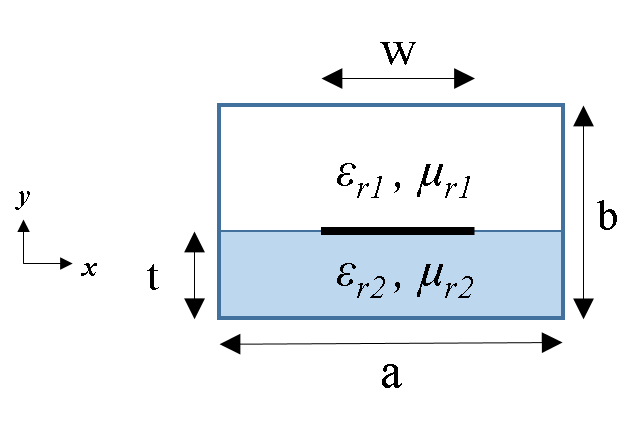
\includegraphics[width=0.5\columnwidth]{./img/rectangular_inhomo_strip/geometry.png}
	\caption{Geometry of partially filled rectangular waveguide. }
	\label{fig:rect_inhomo_strip_geom}
\end{figure}

\newif\ifdisplayspuriousmodestrip
\displayspuriousmodestripfalse

\begin{figure}[htbp]
	\centering
	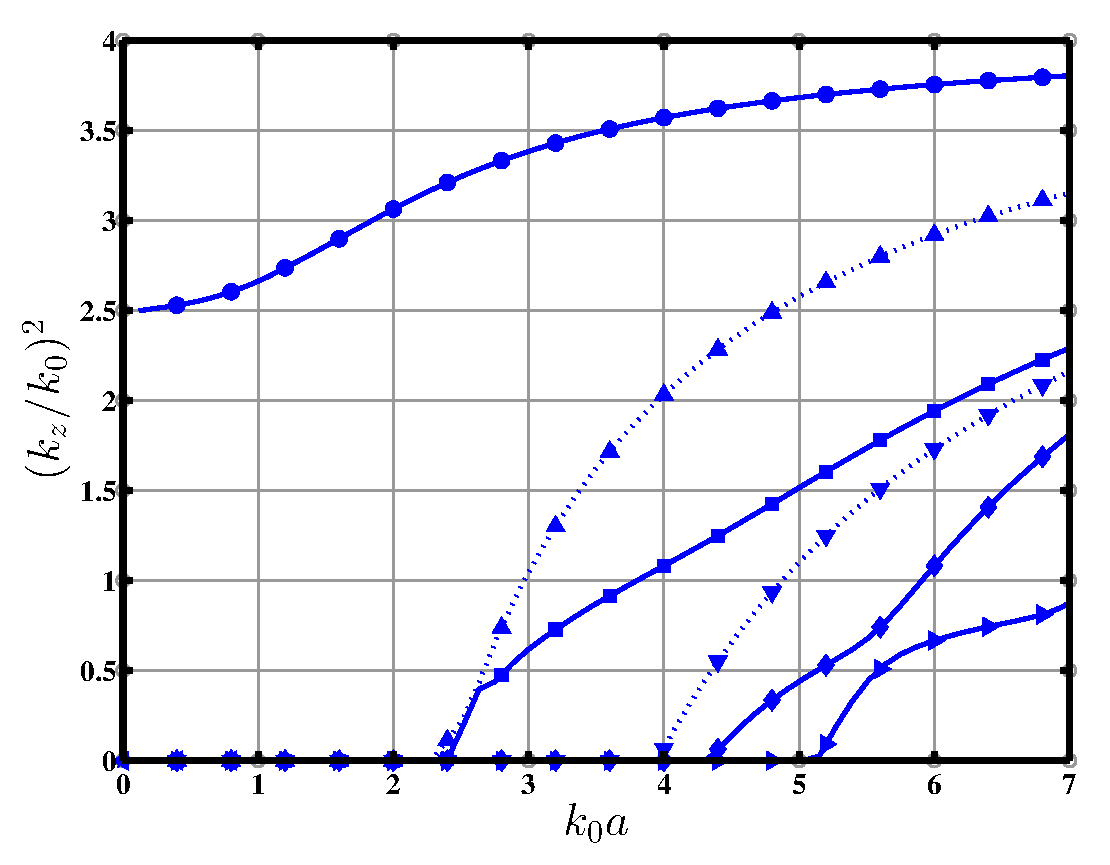
\includegraphics[width=\defaultfigurewidth]{./img/rectangular_inhomo_strip/dispersion.eps}
	\caption{Dispersion curves for a homogeneous cylindrical waveguide. Solid line: Data in \cite{na_JinJM_JinJM_2014_finite_element} \ifdisplayspuriousmodestrip by placing a PMC symmetric plane \fi; \ifdisplayspuriousmodestrip dash line: see text; \fi symbols: numerical solution ($b=a/2$, $t=b/2$, $w=b$, $\mu_{r1}=\mu_{r2}=\epsilon_{r1} = 1$, $\epsilon_{r2} = 4$).}
	\label{fig:rect_inhomo_strip_dispersion}
\end{figure}


\section{Inhomogeneous Transmission Line}
The last section demonstrate a common transmission line used on modern silicon-based chip. The metal-insulator-semiconductor (MIS) structure is has become popular as a basic wave conducting structure recently due to the development of RFIC and millimeter wave IC. This transmission utilizes the metal layer of the chip, and the backside metal of the substrate. However, aside from the traditional microstrip line, an additional layer of insulator, usually made of silicon dioxide, is formed between the microstrip and the silicon substrate, as shown in Fig.~\ref{fig:mis_geom}.\\

\begin{figure}[htbp]
	\centering
	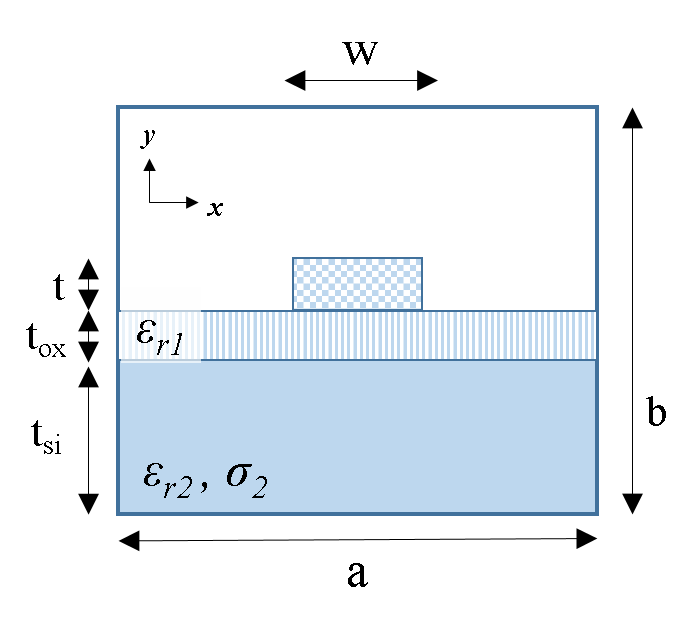
\includegraphics[width=0.5\columnwidth]{./img/mis/geometry.png}
	\caption{Geometry of MIS transmission line. }
	\label{fig:mis_geom}
\end{figure}

For the fundamental mode, three modes are categorized. 1) Slow wave mode: the lossy silicon is considered as a good conductor, the electric field are confined in insulator. 2) Quasi-TEM mode: while the loss of silicon is moderate and frequency is high enough, the displacement current penetrate the silicon substrate, reaching the ground plane, and form quasi-TEM mode. The slow wave factor decreases. 3) when frequency is high with highly lossy silicon, the thickness of substrate is large compared to the skin depth of silicon. The lossy silicon still considered a moderate ground plane. The slow wave factor remains. For complete analysis, see \cite{ITMTT_KiangJF_KiangJF_1996_quasitem_analysis,ITMTT_WilliamsDF_WilliamsDF_1999_metalinsulatorsemiconductor_transmission}. \\

To truncate the computational domain, the out-most boundaries of the MIS is enclosed by PEC wall. The size of the PEC box is $a=8t_{Si}$ and $b=4t_{Si}$. \\

\begin{figure}[htbp]
	\centering
	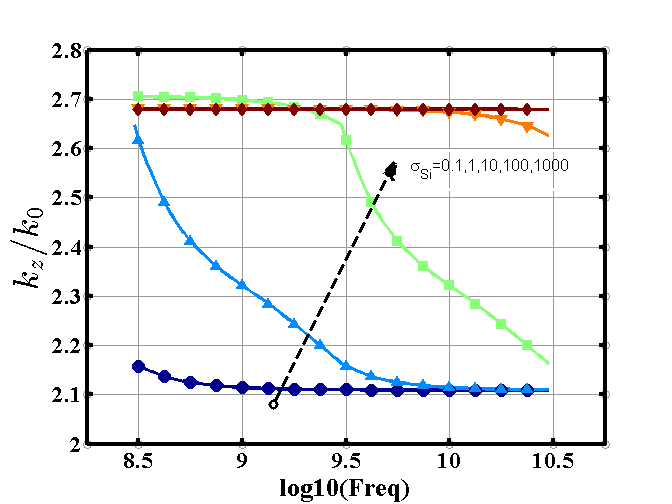
\includegraphics[width=\defaultfigurewidth]{./img/mis/mis_disp.png}
	\caption{Slow wave factor of fundamental mode of MIS with different loss of silicon. Circle: ($\sigma_2=0.1 \mathrm{ mho/m}$);triangle up: ($\sigma_2=1 \mathrm{ mho/m}$); triangle right:($\sigma_2=10 \mathrm{ mho/m}$);triangle down: ($\sigma_2=100 \mathrm{ mho/m}$); diamond: ($\sigma_2=1000 \mathrm{ mho/m}$). ($t=t_{ox}=1\mathrm{um}$, $w=2\mathrm{um}$, $t_{Si}=5\mathrm{um}$, $\epsilon_{r1} = 4$, $\epsilon_{r2} = 11.9$).}
	\label{fig:mis_dispersion}
\end{figure}

Fig.~\ref{fig:mis_dispersion} demonstrate the slow wave factor $k_z/k_0$ of five silicon substrate with different loss, $\sigma_{Si}=0.1,1,10,100,1000$. One can clearly see the transition from slow-wave mode to quasi-TEM mode when the loss of silicon is small, while for highly lossy silicon, the SWF remains the same as frequency increases. This result suggests that MIS with higher lossy silicon may be less dispersive than lossless one. This concluded the result in \cite{OC_XiaoJ_LiS_2012_lowloss_metalinsulatorsemiconductor}.

\section{Conclusion}
In this paper, we use the vector electric field formulation, combined with both edge and element basis, to analyze several type of waveguide structure. Both homogeneous and inhomogeneous  waveguide shows a good agreement to the analytic solution. In addition, the slow wave factors of MIS structure are analyzed with different substrate loss. The transitions from slow wave mode to quasi-TEM mode or skip-depth mode can be clearly observed. 

% =============  Reference Section ==============

\bibliographystyle{IEEEtran}
\bibliography{IEEEabrv,F:/SoftwarePC/AutoupdateZoteroLibrary}

%\begin{thebibliography}{99}	
%
%\end{thebibliography}


\end{document}

